\documentclass[letterpaper, 10 pt, conference]{ieeeconf}

\IEEEoverridecommandlockouts
\overrideIEEEmargins

\usepackage{amsmath}
\usepackage{amssymb}
\usepackage{float}
\usepackage[margin=1in]{geometry}
\usepackage{graphicx}
\usepackage{siunitx}

\title{Project Report: Quadrotor Planning and Control}
\author{Team 123: Benjamin Franklin, Leonhard Euler}

\begin{document}
\maketitle

%%%%%%%%%%%%%%%%%%%%%%%%%%%%%%%%%%%%%%%%%%%%%%%%%%%%%%%%%%%%%%%%%%%%%%%%%%%%%%%%
% \begin{abstract}
% Abstract optional.
% \end{abstract}

%%%%%%%%%%%%%%%%%%%%%%%%%%%%%%%%%%%%%%%%%%%%%%%%%%%%%%%%%%%%%%%%%%%%%%%%%%%%%%%%
\section{Introduction and System Overview}

Introduce the project goals and experimental system.

%%%%%%%%%%%%%%%%%%%%%%%%%%%%%%%%%%%%%%%%%%%%%%%%%%%%%%%%%%%%%%%%%%%%%%%%%%%%%%%%
\section{Controller}

Describe the implementation and performance of your tracking controller.
An example of including a figure is shown in Fig. \ref{fig:example_figure}.

% Example figure
\begin{figure}[h]
  \centering
    % replace sample_figure with your image file name in this folder
    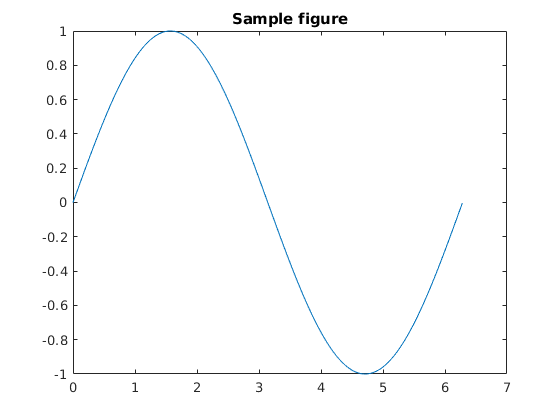
\includegraphics[width=\linewidth]{sample_figure}
  \caption{Figures should have captions.}
  \label{fig:example_figure}
\end{figure}

%%%%%%%%%%%%%%%%%%%%%%%%%%%%%%%%%%%%%%%%%%%%%%%%%%%%%%%%%%%%%%%%%%%%%%%%%%%%%%%%
\section{Trajectory Generator}

Describe the implementation and performance of your trajectory generator.
A simple equation is show in Eqn. \ref{eqn:simple}.

\begin{align}
-1 = e^{i \pi}
\label{eqn:simple}
\end{align}

A matrix equation is shown in Eqn. \ref{eqn:matrix}.

\begin{align}
\begin{bmatrix}
0 & 0 & 0 & 0 & 0 & 1 \\
t_1^5 & t_1^4 & t_1^3 & t_1^2 & t_1^1 & 1
\end{bmatrix}
\begin{bmatrix}
c_5 \\ c_4 \\ c_3 \\ c_2 \\ c_1 \\ c_0 
\end{bmatrix}
=
\begin{bmatrix}
p(0) \\
p(t_1)
\end{bmatrix}
\label{eqn:matrix}
\end{align}

%%%%%%%%%%%%%%%%%%%%%%%%%%%%%%%%%%%%%%%%%%%%%%%%%%%%%%%%%%%%%%%%%%%%%%%%%%%%%%%%
\section{Maze Flight Experiments}

Report your experimental results flying the maze using your planner, trajectory generator, and controller.
Table \ref{tab:simple_table} shows how to create a simple table.

% Example table
\begin{table}[h]
  \centering
  \begin{tabular}{c|c|c}
    a & b & c \\
    \hline
    1 & 2 & 3 \\
    4 & 5 & 6
  \end{tabular}
  \caption{Caption for a table.}
  \label{tab:simple_table}
\end{table}

%%%%%%%%%%%%%%%%%%%%%%%%%%%%%%%%%%%%%%%%%%%%%%%%%%%%%%%%%%%%%%%%%%%%%%%%%%%%%%%%
% \section{Conclusion}
% Conclusion optional.

\end{document}
